% SIGMOD research submission: ACM two-column, anonymous review format.
\documentclass[sigconf,review,anonymous]{acmart}

% Submission-only settings; replace with ACM metadata for the final version.
\setcopyright{none}
\settopmatter{printacmref=false}
\renewcommand{\footnotetextcopyrightpermission}[1]{}
\acmDOI{}
\acmISBN{}
\acmConference{}{}{}
\acmYear{}
\copyrightyear{}

% acmart already loads amsmath, booktabs, graphicx, and hyperref.
% Add shared commands and ACM-approved packages here as needed.
\newcommand{\systemname}{\textsc{SystemName}}


\title{Working Title: Natural Language to SQL}

% Add real authors and affiliations only when preparing the final version.
\author{Anonymous Author(s)}

\begin{document}

\begin{abstract}
  \textit{
    Recent advances in text-to-SQL, particularly on challenging benchmarks such as BIRD, are dominated by one-fits-all pipelines: 
    every natural-language question—regardless of its difficulty—is processed by the same elaborate workflow of schema retrieval, 
    decomposition, multi-candidate generation, iterative repair and selection. Since single-pass generation remains unreliable on 
    complex questions, state-of-the-art systems increasingly rely on test-time scaling—sampling many candidates or invoking 
    multiple collaborating agents—to secure accuracy gains.
    This strategy incurs significant waste in cost and latency. We present **DataGallery-Text2SQL**, a text-to-SQL system built on 
    two complementary ideas. 
    First, a *routing strategy* estimates the difficulty of each incoming question and dispatches it to appropriate execution 
    paths, reserving expensive scaled inference for the questions in need. Second, a \bf{self-evolving checker} automatically 
    generates and continually improves SQL verification criteria from execution feedback, replacing hand-crafted candidate-selection heuristics.
}


\end{abstract}

% Replace with the paper's actual CCS concepts before submission.
\keywords{natural language interfaces, text-to-SQL, data management}

\maketitle

\section{Introduction}
\label{sec:introduction}
\textit{TODO: Motivate the problem, explain the limitations of existing
approaches, and summarize the contributions.}

\section{Background and Problem Formulation}
\label{sec:background}
\textit{TODO: Introduce the necessary background, notation, inputs,
outputs, and assumptions.}

\section{Method}
\label{sec:method}

\subsection{Overview}
\label{sec:overview}

Given a natural-language question $Q$ and a target database $D$, text-to-SQL aims
to produce a query $S^{*}$ that executes on $D$ and returns the correct result set.
LLM-based solutions largely adopt a one-fits-all pipeline, applying the same
procedure to every question and raising accuracy by sampling many SQL candidates for
selection. This scaling exhibits diminishing returns: accuracy gains flatten as the
sample count grows, whereas token and latency costs increase markedly even for simple
questions. \systemname{} replaces this indiscriminate scaling with two mechanisms:
difficulty-conditioned dynamic routing and self-evolving validation.

\paragraph{Difficulty-Conditioned Dynamic Routing.}
Routing configures three modules of the pipeline according to a difficulty probe
$d(Q)$: (i) which recall paths Schema Linking activates, (ii) which generation paths
Generator activates, and (iii) how many candidate clusters the Selector chooses among.
The candidate pool therefore varies with difficulty: simple questions receive a compact
pool without broad exploration, moderate questions a pool whose exploration range spans
plausible solutions, and challenging questions a pool generated only from the most
reasoning-intensive paths.

\paragraph{Self-Evolving Validation.}
We design validation as a chain of checkers, so that an RSI agent can evolve any single
checker independently against one error type or a scenario preference; in combination,
the chain covers the whole scenario and all common error types. Two generic checkers
anchor both ends of the chain, verifying syntax validity and execution results, while
the RSI agent extends or modifies the intermediate checkers in the overall evolution loop.
Each iteration revises one checker, re-executes the pipeline on the development set, and
analyzes the resulting errors to direct the next revision. Discovery and resolution of
these issues thus no longer require manual analysis, which facilitates migration to a new
application scenario.

Figure~\ref{fig:overview} presents the framework in two complementary views. The
execution view (right) describes the online path of a single request: Schema Linking
retrieves the relevant tables and columns, Generator produces candidate SQL through
multiple reasoning paths in parallel, Validator detects and repairs the candidates, and
Selector returns the final query $S^{*}$. The development view (left) describes how the
guidelines used by Generator and Validator are produced. An offline semantic modeling
pass, run once per database and shared by both views, builds the semantic layer that
every query on that database reuses.

The following subsections describe the principal modules and mechanisms of the framework.

\begin{figure*}[t]
\centering
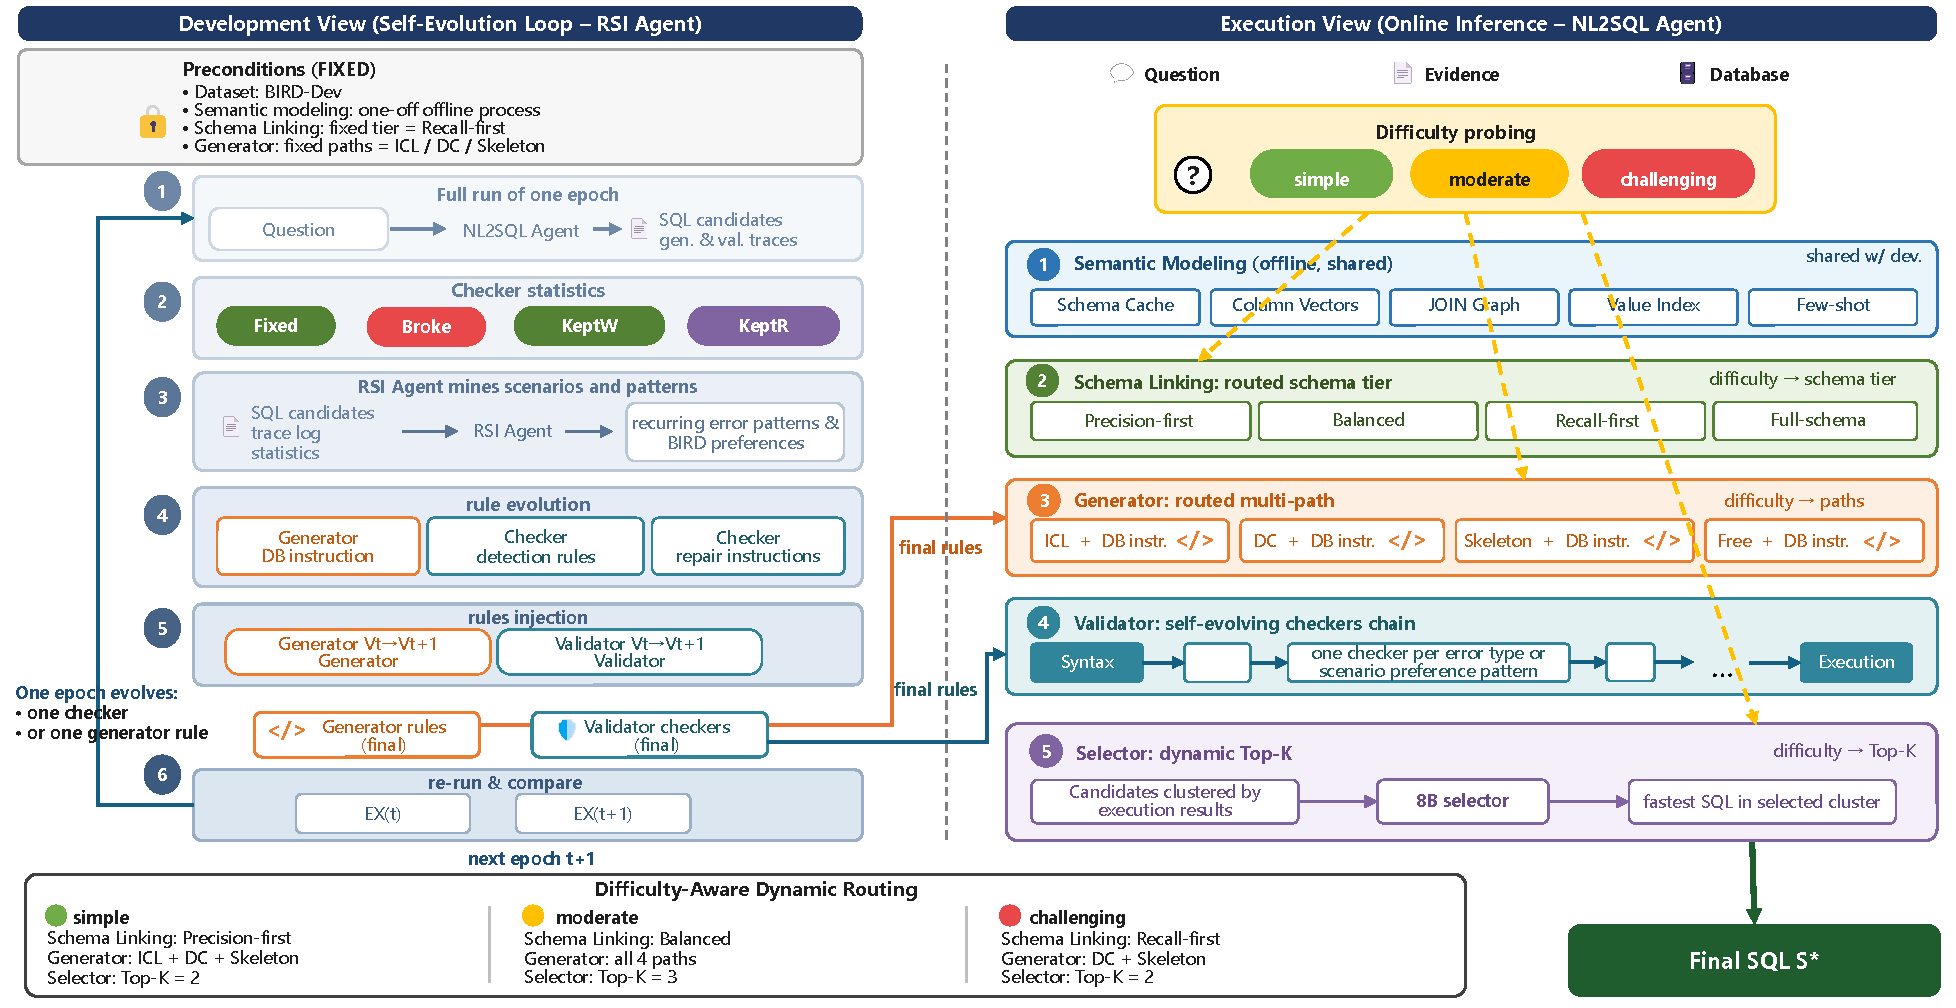
\includegraphics[width=\textwidth]{figures/figure1.pdf}
\Description{Two side-by-side panels. The left panel is the development view, a six-step
self-evolution loop that starts from a fixed development configuration and repeatedly
classifies checker outcomes, mines error scenarios, evolves generator and validator
rules, and re-runs the pipeline. The right panel is the execution view, where a
difficulty probe routes a question through semantic modeling, schema linking, multi-path
generation, a self-evolving checker chain, and a dynamic Top-K selector. A routing table
beneath the panels lists the schema tier, generation paths, and Top-K per difficulty level.}
\caption{Overview of \systemname{}.}
\label{fig:overview}
\end{figure*}

\subsection{Semantic Modeling}
\label{sec:semantic-modeling}

Enterprise data environments often contain hundreds of tables and hundreds of millions
of rows. BIRD~\cite{li2023bird}, a benchmark aligned with such environments, operates at
this scale. Frequent probing of the database and its related semantic corpora during
inference incurs prohibitive costs in tokens and latency, and adds load to the production
environment. \systemname{} therefore replaces this probing with an LLM-friendly semantic
layer built once offline and queried directly.

Semantic modeling builds the semantic layer from four sources: the database schema,
database description files, sampled column values, and query logs, the last approximated
in BIRD by the training set's question-SQL pairs. The process extracts table and column
semantics, including enumerated values and derived metrics, and links tables, columns,
and JOIN relations into a graph. It also indexes table and column entries, sampled values,
and few-shot SQL in a vector retrieval system. Together, they form the semantic layer
queried by Schema Linking during inference.

\subsection{Multi-Path Dynamic Schema Linking}
\label{sec:schema-linking}

\begin{table*}[t]
\centering
\caption{The seven recall paths of Schema Linking.}
\label{tab:recall-paths}
\small
\begin{tabular}{@{}l p{0.66\textwidth}@{}}
\toprule
Recall path & Mechanism \\
\midrule
Column semantic matching & Vector retrieval over column descriptions, queried by the extracted keywords. \\
Column LLM matching & LLM selects columns from descriptions, value profiles, and schema relations. \\
Column-value LSH matching & Lexical retrieval over an LSH index of column values. \\
Column-value vector matching & Semantic retrieval over a vector index of column values. \\
Enumerated-value vector matching & Semantic retrieval over a vector index of enumerated value descriptions. \\
SQL reverse linking & LLM drafts a SQL query and extracts the tables and columns it
  references. \\
JOIN graph expansion & Multi-hop traversal of the JOIN graph, adding the tables and foreign keys that
  connect the recalled tables. \\
\bottomrule
\end{tabular}
\end{table*}

Schema Linking decides which tables and columns enter the context passed to SQL
generation, and thus whether generation starts from an accurate scope; it therefore bounds
attainable accuracy. Improving its precision and recall is a main line of
text-to-SQL research, from decoupling schema linking~\cite{li2023resdsql} and pruning
industrial-scale schemas~\cite{talaei2024chess} to bidirectional
linking~\cite{cao2024rslsql}, all relying on a static strategy. \systemname{} instead
implements a dynamic seven-path recall pipeline (Table~\ref{tab:recall-paths}), each
path switchable independently; their on/off configuration sets the recall--precision
trade-off of the output context and is adjusted online to the question difficulty. It
begins with a Perceptor that parses the question into keywords for table and column
matching.

Among the seven recall paths, SQL reverse linking warrants additional explanation. It
follows from how LLMs are trained: pretraining corpora are rich in SQL generation but
rarely annotate schema linking, so LLM-based direct matching lacks support, whereas
drafting a SQL query and parsing its references matches the training distribution. The
path therefore complements the direct-matching paths, recovering the columns they miss
(Section~\ref{sec:exp-schema-linking}), and its drafted SQL serves as the difficulty probe
of Section~\ref{sec:generation}.

We enumerate all non-empty on/off combinations of the seven paths on the BIRD
development set, obtaining $2^{7}-1=127$ configurations, and rank them by Strict Column
Recall, the fraction of questions for which all ground-truth columns are recalled, with
Micro Precision as the tie-breaker. Reading this ranking along the recall--precision
trade-off, we select three representative tiers plus a full-schema fallback:

\begingroup
\setlength{\topsep}{6pt}
\setlength{\partopsep}{0pt}
\begin{itemize}
  \setlength{\itemsep}{1pt}
  \setlength{\parsep}{0pt}
  \item \textbf{Recall-first} enables all seven paths, favoring recall at the cost of
    context size.
  \item \textbf{Balanced} disables enumerated-value vector matching and JOIN graph
    expansion, the two most redundant paths.
  \item \textbf{Precision-first} retains only column LLM matching and SQL reverse linking,
    sacrificing join and value coverage.
  \item \textbf{Full-schema} keeps every table and column, bypassing all paths as the
    fallback.
\end{itemize}
\endgroup

The per-configuration and per-tier recall and precision of these tiers are reported in
Section~\ref{sec:exp-schema-linking}. The applicable tier is chosen per question by the
difficulty probe $d(Q)$ (Section~\ref{sec:generation}), so that the same seven-path
pipeline yields a leaner or a richer schema context as the question difficulty varies.

That context is then rendered in a DDL semantic format (Appendix~\ref{app:ddl}):
\texttt{CREATE TABLE} statements preserve the schema structure, primary and foreign key
constraints declare JOIN hints explicitly, and column comments embed descriptions, value
samples (\texttt{Examples}), and matched enumerated values with explanation
(\texttt{Matched values}), enabling the LLM to interpret the schema more completely.

\subsection{Difficulty-Conditioned Multi-Path Generation}
\label{sec:generation}

SQL generation follows the N-version programming principle~\cite{chen1978nversion}:
the four paths act as independent versions that solve the same question $Q$ with
optional evidence $E$, and they pool their outputs for selection. Diversity therefore
stems from the paths rather than from repeatedly sampling a single path, as
self-consistency does~\cite{wang2023selfconsistency}. Table~\ref{tab:generation} lists
the four paths, which guide SQL generation through different reasoning strategies: the
first three follow in-context learning, recursive decomposition (as in least-to-most
prompting~\cite{zhou2023leasttomost}), and skeleton-first generation, whereas free
exploration leaves the reasoning strategy unconstrained and serves as the fallback path.

\begin{table*}[t]
\centering
\caption{Generation paths (top) and difficulty-conditioned routing (bottom).}
\label{tab:generation}
\small
\begin{tabular}{@{}l l p{0.56\textwidth}@{}}
\toprule
Path & Notation & Reasoning strategy \\
\midrule
Few-shot ICL & $r_\text{icl}$ & Guides the LLM to learn SQL structure and semantic
  mapping from cross-domain question--SQL demonstrations. \\
Divide-and-conquer & $r_\text{dc}$ & Recursively decomposes the question, solves each part,
  and assembles them bottom-up. \\
Skeleton-first & $r_\text{skel}$ & Drafts the clause skeleton, then fills its slots with
  schema elements, literals, and operators. \\
Free exploration & $r_\text{free}$ & Leaves the reasoning strategy unconstrained and serves as
  the fallback path. \\
\bottomrule
\end{tabular}

\vspace{5pt}
\begin{tabular}{@{}l l l@{}}
\toprule
Difficulty $d(Q)$ & Schema tier $\mathrm{Sch}(Q)$ & Active paths $\mathcal{R}(Q)$ \\
\midrule
simple & Precision-first & $\{r_\text{icl}, r_\text{dc}, r_\text{skel}\}$ \\
moderate & Balanced & $\{r_\text{icl}, r_\text{dc}, r_\text{skel}, r_\text{free}\}$ \\
challenging & Recall-first & $\{r_\text{dc}, r_\text{skel}\}$ \\
\bottomrule
\end{tabular}
\end{table*}

To maximize SQL generation accuracy, \systemname{} configures the active paths and the
schema context per question, driven by a difficulty probe $d(Q)$ whose value is one of
\emph{simple}, \emph{moderate}, and \emph{challenging}. The probe has two interchangeable
sources: the labels released with the benchmark, and a structural probe computed from the
draft SQL of SQL reverse linking (Section~\ref{sec:schema-linking}). The latter applies
Spider's hardness criteria~\cite{yu2018spider}, counting query components, nesting depth,
explicit joins, and aggregate or set operations. Both yield comparable routing decisions
on the BIRD development set; since BIRD annotates every question, all BIRD evaluations in
this paper use the benchmark labels.

Given $d(Q)$, routing assigns each question a schema tier $\mathrm{Sch}(Q)$ and an active
path set $\mathcal{R}(Q)$ (Table~\ref{tab:generation}, bottom); each active path then
receives its own schema:
\begin{equation}
\mathrm{Sch}_r =
\underbrace{
\begin{cases}
\text{Full-schema}, & r = r_\text{free},\\
\mathrm{Sch}(Q), & \text{otherwise},
\end{cases}
}_{\mathrm{PathSchema}(r,\,\mathrm{Sch}(Q))}
\tag{1}
\end{equation}
where $\mathrm{Sch}(Q)$ is the question-level context returned by Schema Linking
(Section~\ref{sec:schema-linking}).

These assignments derive from per-difficulty combination studies of the recall and
generation paths (Sections~\ref{sec:exp-schema-linking} and~\ref{sec:exp-generation}).
Simple questions need a precision-leaning schema and only three reasoning-guided paths,
keeping a compact SQL candidate pool with the correct SQL concentrated for easy selection.
Moderate questions balance schema precision against recall and add free exploration,
raising the accuracy ceiling of the pool. Challenging questions favor schema recall yet
run only divide-and-conquer and skeleton-first, removing the noise of the other two
paths. The routing thus maximizes generation accuracy and candidate pool purity for each
difficulty, which benefits the subsequent Selector.

To bound token consumption and latency, the pool grows in two stages with per-path
budgets $m$ and $n$, and the second stage is invoked only when needed. In stage one, each
active path produces $m$ candidates, and only those that pass validation enter
$\mathcal{C}$. The Single check then tests whether all pooled candidates execute to the
same result set. This early exit mirrors adaptive
stopping~\cite{aggarwal2023adaptiveconsistency}, with executable result equivalence
replacing answer voting as the stability criterion. If the check fails, stage two extends
every path to $n$ candidates under the same validation.

\begin{algorithm}[t]
\caption{Difficulty-routed two-stage generation.}
\label{alg:generation}
\begin{algorithmic}[1]
\Require $Q$, $E$, $d(Q)$; $m$, $n$ ($m < n$)
\Ensure validated pool $\mathcal{C}$
\State $(\mathit{tier}, \mathcal{R}) \gets \mathrm{Route}(d(Q))$
\State $\mathrm{Sch}(Q) \gets \mathrm{Link}(Q, E, \mathit{tier})$
\State $\mathcal{C} \gets \emptyset$
\For{$r \in \mathcal{R}$} \Comment{stage one}
  \State $\mathrm{Sch}_r \gets \mathrm{PathSchema}(r, \mathrm{Sch}(Q))$
  \For{$i = 1$ to $m$}
    \State $s \gets \mathrm{Validate}(\mathrm{Gen}_r(Q, E, \mathrm{Sch}_r))$
    \If{$\mathrm{Valid}(s)$}
      \State $\mathcal{C} \gets \mathcal{C} \cup \{(s, r)\}$
    \EndIf
  \EndFor
\EndFor
\If{$\mathcal{C} \neq \emptyset$ \textbf{and} $\mathrm{Single}(\mathcal{C})$}
  \State \Return $\mathcal{C}$
\EndIf
\For{$r \in \mathcal{R}$} \Comment{stage two}
  \State $\mathrm{Sch}_r \gets \mathrm{PathSchema}(r, \mathrm{Sch}(Q))$
  \For{$i = m+1$ to $n$}
    \State $s \gets \mathrm{Validate}(\mathrm{Gen}_r(Q, E, \mathrm{Sch}_r))$
    \If{$\mathrm{Valid}(s)$}
      \State $\mathcal{C} \gets \mathcal{C} \cup \{(s, r)\}$
    \EndIf
  \EndFor
\EndFor
\State \Return $\mathcal{C}$
\end{algorithmic}
\end{algorithm}

\subsection{Self-Evolving Validator Chain}
\label{sec:validator}

\begin{zhoutline}
\begin{itemize}
\item 介绍：把校验外化为确定性 Checker 链，一头一尾为语法与执行结果校验，中间按子句与语义场景串行扩充，命中即给指令、由 LLM 定向修复。
\item 公式（式 2、式 3）：演进算子依据 Fixed、Broke、KeptW、KeptR 四类统计，收紧或放宽检测谓词、细化修复指令，或派生新 Checker。
\item 算法（算法 3）：单目标串行迭代，修改需通过全量 NoRegression 回归方可生效。
\end{itemize}
\end{zhoutline}

\subsection{Dynamic Top-K Selector}
\label{sec:selector}

\begin{zhoutline}
\begin{itemize}
\item 介绍：8B 概率选择器，候选先按执行结果聚类，仅在 Top-K 个簇代表上打分；单簇占满时短路，零模型调用。
\item 公式（式 4、式 5）：给出选择规则，并把 K 与回路组合绑定，四路全开取 3，不含自由探索取 2。
\end{itemize}
\end{zhoutline}

\section{Experimental Evaluation}
\label{sec:experiments}
\textit{TODO: Define research questions, datasets, baselines, metrics,
experimental settings, main results, and ablation studies.}

\section{Related Work}
\label{sec:related-work}
\textit{TODO: Discuss relevant research and position the contributions.}

\textit{Template citation (replace): ACM article template~\cite{acmart}.}

\section{Conclusion}
\label{sec:conclusion}
\textit{TODO: Summarize the key findings and discuss future work.}


\bibliographystyle{ACM-Reference-Format}
\bibliography{references}

% Draft appendix; SIGMOD review appendices move to a separate PDF at submission.
\appendix
\section{An Example of the DDL Semantic Format}
\label{app:ddl}

\begin{figure*}[!t]
\centering
\begin{lstlisting}
CREATE TABLE frpm (
  `CDSCode` TEXT, -- COMMENT "CDS code. Examples: ['01100170109835', '01100170112607', '01100170118489']"
  `District Code` INTEGER, -- COMMENT "district code. Matched values: ['61333']. Examples: ['10017', '31609']"
  `School Code` TEXT, -- COMMENT "school code. Examples: ['0109835', '0112607', '0118489']"
  `District Name` TEXT, -- COMMENT "district name. Matched values: ['National Elementary', 'Center Joint Unified', 'Orange Center']"
  `School Name` TEXT, -- COMMENT "school name. Matched values: ['Special Education', 'Center Middle', 'District Office']"
  `District Type` TEXT, -- COMMENT "district type. Matched values: ['Unified School District', 'High School District', 'State Special Schools']"
  `School Type` TEXT, -- COMMENT "school type. Matched values: ['Special Education Schools (Public)', 'State Special Schools', 'District Community Day Schools']"
  `Educational Option Type` TEXT, -- COMMENT "educational option type. Matched values: ['District Special Education Consortia School', 'Special Education School', 'State Special School']"
  `NSLP Provision Status` TEXT, -- COMMENT "National School Lunch Program provision status. Matched values: ['Provision 1', 'Provision 3', 'Provision 2']"
  `Charter School Number` TEXT, -- COMMENT "charter school number. Matched values: ['0616', '0613', '0660']"
  `Low Grade` TEXT, -- COMMENT "low grade. Matched values: ['6', 'Adult', '1']"
  `High Grade` TEXT, -- COMMENT "high grade. Matched values: ['6', 'Adult', 'Post Secondary']"
  `Free Meal Count (K-12)` REAL, -- COMMENT "free meal count for K-12 students. Examples: ['565.0', '186.0', '134.0']"
  `Enrollment (Ages 5-17)` REAL, -- COMMENT "enrollment count for ages 5 to 17. Examples: ['1070.0', '376.0', '230.0']"
  `Free Meal Count (Ages 5-17)` REAL, -- COMMENT "free meal count for ages 5-17. Examples: ['553.0', '182.0', '128.0']"
  `FRPM Count (Ages 5-17)` REAL, -- COMMENT "FRPM count for ages 5-17. Examples: ['702.0', '182.0', '168.0']"
  PRIMARY KEY (`CDSCode`)
  FOREIGN KEY (`CDSCode`) REFERENCES schools(`CDSCode`)
);

CREATE TABLE satscores (
  `cds` TEXT, -- COMMENT "California Department Schools. Examples: ['10101080000000', '10101080109991', '10101080111682']"
  `sname` TEXT, -- COMMENT "school name. Matched values: ['Center High', 'The Education Corps', 'Prospect Education Center']"
  `enroll12` INTEGER, -- COMMENT "enrollment count for grades 1 to 12. Examples: ['398', '62', '75']"
  PRIMARY KEY (`cds`)
  FOREIGN KEY (`cds`) REFERENCES schools(`CDSCode`)
);

CREATE TABLE schools (
  `CDSCode` TEXT, -- COMMENT "CDSCode. Examples: ['01100170000000', '01100170109835', '01100170112607']"
  `NCESDist` TEXT, -- COMMENT "NCES school district identification number. Matched values: ['0613360', '0601336']. Examples: ['0691051']"
  `NCESSchool` TEXT, -- COMMENT "NCES school identification number. Examples: ['10546', '10947', '12283']"
  `StatusType` TEXT, -- COMMENT "district status type. Matched values: ['Pending', 'Closed', 'Active']"
  `District` TEXT, -- COMMENT "district identifier. Matched values: ['National Elementary', 'Center Joint Unified', 'Center Joint Elementary']"
  `School` TEXT, -- COMMENT "school name. Matched values: ['Special Education', 'Special Education Preschool', 'Alternative Education/Independent Study']"
  `Phone` TEXT, -- COMMENT "phone number. Matched values: ['(559) 233-0706', '(661) 837-6060', '(661) 636-4621']"
  `Ext` TEXT, -- COMMENT "phone number extension. Examples: ['130', '1240', '1200']"
  `CharterNum` TEXT, -- COMMENT "charter school number. Matched values: ['0616', '0613', '0610']"
  `EdOpsCode` TEXT, -- COMMENT "education option type description. Matched values: ['SPECON'(District Consortia Special Education School), 'SPEC'(Special Education School), 'CON'(Continuation School)]"
  `EdOpsName` TEXT, -- COMMENT "educational option name. Matched values: ['District Special Education Consortia School', 'Special Education School', 'State Special School']"
  `EILCode` TEXT, -- COMMENT "educational instruction level code. Matched values: ['UG'(Ungraded), 'A'(Adult), 'INTMIDJR'(Intermediate/Middle/Junior High)]"
  `EILName` TEXT, -- COMMENT "educational instruction level name. Matched values: ['High School', 'Preschool', 'Intermediate/Middle/Junior High']"
  `GSoffered` TEXT, -- COMMENT "grade span offered. Matched values: ['6-12', '6-10', '6-11']"
  `GSserved` TEXT, -- COMMENT "grade span served. Matched values: ['6-12', '6-10', '6-11']"
  PRIMARY KEY (`CDSCode`)
);
\end{lstlisting}
\caption{The DDL semantic context for question 74 on \texttt{california\_schools}.}
\label{fig:ddl-context}
\end{figure*}

Schema Linking returns a DDL context in which each recalled table keeps its selected
columns and primary and foreign keys, and each column comment carries the description,
sampled values (\texttt{Examples}), and the matched values (\texttt{Matched\ values}). For
an enumerated column, each matched value takes the form \emph{value (description)}, e.g.,
\texttt{\textquotesingle UG\textquotesingle} (Ungraded). The example below is the Schema
Linking output for question~74 of the BIRD development set (difficulty moderate).

\begin{quote}
\textit{Question.} What is the lowest grade for the District Special Education Consortia
School with National Center for Educational Statistics school district identification
number of 0613360?
\end{quote}

The context in Figure~\ref{fig:ddl-context} recalls the columns the question needs:
\texttt{Low Grade}, \texttt{NCESDist} (\texttt{0613360}), \texttt{EdOpsCode}, and the
JOIN key \texttt{CDSCode}. Its foreign key declarations give explicit JOIN evidence
between \texttt{frpm} and \texttt{schools}, and the matched value
\texttt{\textquotesingle SPECON\textquotesingle} (District Consortia Special Education
School) maps District Special Education Consortia School in the question to a filter on
\texttt{EdOpsCode}.


\end{document}
